% Options for packages loaded elsewhere
% Options for packages loaded elsewhere
\PassOptionsToPackage{unicode}{hyperref}
\PassOptionsToPackage{hyphens}{url}
%
\documentclass[
  10pt,
  ignorenonframetext,
  aspectratio=169,
]{beamer}
\newif\ifbibliography
\usepackage{pgfpages}
\setbeamertemplate{caption}[numbered]
\setbeamertemplate{caption label separator}{: }
\setbeamercolor{caption name}{fg=normal text.fg}
\beamertemplatenavigationsymbolsempty
% remove section numbering
\setbeamertemplate{part page}{
  \centering
  \begin{beamercolorbox}[sep=16pt,center]{part title}
    \usebeamerfont{part title}\insertpart\par
  \end{beamercolorbox}
}
\setbeamertemplate{section page}{
  \centering
  \begin{beamercolorbox}[sep=12pt,center]{section title}
    \usebeamerfont{section title}\insertsection\par
  \end{beamercolorbox}
}
\setbeamertemplate{subsection page}{
  \centering
  \begin{beamercolorbox}[sep=8pt,center]{subsection title}
    \usebeamerfont{subsection title}\insertsubsection\par
  \end{beamercolorbox}
}
% Prevent slide breaks in the middle of a paragraph
\widowpenalties 1 10000
\raggedbottom
\AtBeginPart{
  \frame{\partpage}
}
\AtBeginSection{
  \ifbibliography
  \else
    \frame{\sectionpage}
  \fi
}
\AtBeginSubsection{
  \frame{\subsectionpage}
}
\usepackage{iftex}
\ifPDFTeX
  \usepackage[T1]{fontenc}
  \usepackage[utf8]{inputenc}
  \usepackage{textcomp} % provide euro and other symbols
\else % if luatex or xetex
  \usepackage{unicode-math} % this also loads fontspec
  \defaultfontfeatures{Scale=MatchLowercase}
  \defaultfontfeatures[\rmfamily]{Ligatures=TeX,Scale=1}
\fi
\usepackage{lmodern}

\usetheme[]{default}
\ifPDFTeX\else
  % xetex/luatex font selection
\fi
% Use upquote if available, for straight quotes in verbatim environments
\IfFileExists{upquote.sty}{\usepackage{upquote}}{}
\IfFileExists{microtype.sty}{% use microtype if available
  \usepackage[]{microtype}
  \UseMicrotypeSet[protrusion]{basicmath} % disable protrusion for tt fonts
}{}
\makeatletter
\@ifundefined{KOMAClassName}{% if non-KOMA class
  \IfFileExists{parskip.sty}{%
    \usepackage{parskip}
  }{% else
    \setlength{\parindent}{0pt}
    \setlength{\parskip}{6pt plus 2pt minus 1pt}}
}{% if KOMA class
  \KOMAoptions{parskip=half}}
\makeatother

\usepackage{color}
\usepackage{fancyvrb}
\newcommand{\VerbBar}{|}
\newcommand{\VERB}{\Verb[commandchars=\\\{\}]}
\DefineVerbatimEnvironment{Highlighting}{Verbatim}{commandchars=\\\{\}}
% Add ',fontsize=\small' for more characters per line
\newenvironment{Shaded}{}{}
\newcommand{\AlertTok}[1]{\textcolor[rgb]{1.00,0.00,0.00}{\textbf{#1}}}
\newcommand{\AnnotationTok}[1]{\textcolor[rgb]{0.38,0.63,0.69}{\textbf{\textit{#1}}}}
\newcommand{\AttributeTok}[1]{\textcolor[rgb]{0.49,0.56,0.16}{#1}}
\newcommand{\BaseNTok}[1]{\textcolor[rgb]{0.25,0.63,0.44}{#1}}
\newcommand{\BuiltInTok}[1]{\textcolor[rgb]{0.00,0.50,0.00}{#1}}
\newcommand{\CharTok}[1]{\textcolor[rgb]{0.25,0.44,0.63}{#1}}
\newcommand{\CommentTok}[1]{\textcolor[rgb]{0.38,0.63,0.69}{\textit{#1}}}
\newcommand{\CommentVarTok}[1]{\textcolor[rgb]{0.38,0.63,0.69}{\textbf{\textit{#1}}}}
\newcommand{\ConstantTok}[1]{\textcolor[rgb]{0.53,0.00,0.00}{#1}}
\newcommand{\ControlFlowTok}[1]{\textcolor[rgb]{0.00,0.44,0.13}{\textbf{#1}}}
\newcommand{\DataTypeTok}[1]{\textcolor[rgb]{0.56,0.13,0.00}{#1}}
\newcommand{\DecValTok}[1]{\textcolor[rgb]{0.25,0.63,0.44}{#1}}
\newcommand{\DocumentationTok}[1]{\textcolor[rgb]{0.73,0.13,0.13}{\textit{#1}}}
\newcommand{\ErrorTok}[1]{\textcolor[rgb]{1.00,0.00,0.00}{\textbf{#1}}}
\newcommand{\ExtensionTok}[1]{#1}
\newcommand{\FloatTok}[1]{\textcolor[rgb]{0.25,0.63,0.44}{#1}}
\newcommand{\FunctionTok}[1]{\textcolor[rgb]{0.02,0.16,0.49}{#1}}
\newcommand{\ImportTok}[1]{\textcolor[rgb]{0.00,0.50,0.00}{\textbf{#1}}}
\newcommand{\InformationTok}[1]{\textcolor[rgb]{0.38,0.63,0.69}{\textbf{\textit{#1}}}}
\newcommand{\KeywordTok}[1]{\textcolor[rgb]{0.00,0.44,0.13}{\textbf{#1}}}
\newcommand{\NormalTok}[1]{#1}
\newcommand{\OperatorTok}[1]{\textcolor[rgb]{0.40,0.40,0.40}{#1}}
\newcommand{\OtherTok}[1]{\textcolor[rgb]{0.00,0.44,0.13}{#1}}
\newcommand{\PreprocessorTok}[1]{\textcolor[rgb]{0.74,0.48,0.00}{#1}}
\newcommand{\RegionMarkerTok}[1]{#1}
\newcommand{\SpecialCharTok}[1]{\textcolor[rgb]{0.25,0.44,0.63}{#1}}
\newcommand{\SpecialStringTok}[1]{\textcolor[rgb]{0.73,0.40,0.53}{#1}}
\newcommand{\StringTok}[1]{\textcolor[rgb]{0.25,0.44,0.63}{#1}}
\newcommand{\VariableTok}[1]{\textcolor[rgb]{0.10,0.09,0.49}{#1}}
\newcommand{\VerbatimStringTok}[1]{\textcolor[rgb]{0.25,0.44,0.63}{#1}}
\newcommand{\WarningTok}[1]{\textcolor[rgb]{0.38,0.63,0.69}{\textbf{\textit{#1}}}}

\usepackage{longtable,booktabs,array}
\usepackage{calc} % for calculating minipage widths
\usepackage{caption}
% Make caption package work with longtable
\makeatletter
\def\fnum@table{\tablename~\thetable}
\makeatother
\usepackage{graphicx}
\makeatletter
\newsavebox\pandoc@box
\newcommand*\pandocbounded[1]{% scales image to fit in text height/width
  \sbox\pandoc@box{#1}%
  \Gscale@div\@tempa{\textheight}{\dimexpr\ht\pandoc@box+\dp\pandoc@box\relax}%
  \Gscale@div\@tempb{\linewidth}{\wd\pandoc@box}%
  \ifdim\@tempb\p@<\@tempa\p@\let\@tempa\@tempb\fi% select the smaller of both
  \ifdim\@tempa\p@<\p@\scalebox{\@tempa}{\usebox\pandoc@box}%
  \else\usebox{\pandoc@box}%
  \fi%
}
% Set default figure placement to htbp
\def\fps@figure{htbp}
\makeatother





\setlength{\emergencystretch}{3em} % prevent overfull lines

\providecommand{\tightlist}{%
  \setlength{\itemsep}{0pt}\setlength{\parskip}{0pt}}



 


%%
%% Theme for BeamerClass: BHT Corporate Desgign 
%%
%% This theme bases on the theme warsaw. Beside this files, 
%% the corresponding colortheme is required:
%%    - beamercolorthemeBHT for presentations
%%
%% Usually, a beamerclass theme is split in three parts 
%% (inner, outer, color) and a theme file. These parts are
%% combined in this file.
%%
%% 28.09.2022 Beate Navarro
%%

% This program can be redistributed and/or modified under the terms
% of the GNU Public License, version 2.

\ProvidesPackage{beamerthemeBHT}[2009/04/30 V0.5 BHT beamertheme]
%%%%%%%%%%%%%%%%%%%%%%%%%%%%%%%%%%%%%%%%%%%%%%%%%%%%%%%%%
%% Presentation mode
%%
\mode<presentation>

%%%%%%%%%%%%%%%%%%%%%%%%%%%%%%%%%%%%%%%%%%%%%%%%%%%%%%%%%
%% Setting the Base
\useinnertheme[shadow=true]{rounded}
%\useoutertheme{shadow}
%\usecolortheme{BHT}
\usepackage{ifthen}
%\usepackage{minted}
\usepackage{tikz}


\setbeamerfont{block title}{size={\small}}


%\definecolor{FGtext}{RGB}{0,0,0}
\definecolor{FGtext}{RGB}{0.03, 0.27, 0.49}
\xdefinecolor{HKS51}{rgb}{0.03, 0.27, 0.49}          % HKS51, THI blau
\definecolor{THIINF}{HTML}{D7D700}          % HKS51, THI Märzrün
\definecolor{rladiesgray}{HTML}{D3D3D3}

\setbeamercolor{subtitlebar}{fg=HKS51, bg=THIINF}
\setbeamercolor*{title in head/foot}{fg=HKS51, bg=white}
\setbeamercolor*{frametitle}{fg=HKS51, bg=white}
\setbeamercolor*{framesubtitle}{fg=HKS51,bg=white}
\setbeamercolor*{frametitleLogo}{bg=white}
\setbeamercolor*{frametitleLogoDEV}{bg=HKS51!44}
\setbeamercolor*{footline}{fg=HKS51,bg=white}


\setbeamerfont*{section in head/foot}{size=\footnotesize}
\setbeamerfont*{frametitle}{size=\small}%
\setbeamerfont*{sectionnavigationhorizontal}{size=\tiny}
\setbeamerfont{section in toc}{size={\footnotesize}}
\setbeamerfont{subsection in toc}{size={\footnotesize}}

\setbeamercolor{itemize item}{fg=HKS51}
\setbeamercolor{itemize subitem}{fg=HKS51}
\setbeamercolor{itemize subsubitem}{fg=HKS51}
\setbeamertemplate{itemize items}[circle]
\setbeamercolor{enumerate item}{fg=HKS51}
\setbeamercolor{enumerate text}{fg=HKS51}

 \setbeamercolor{normal text}{fg=HKS51}
 \usebeamercolor[fg]{normal text}



%%%%%%%%%%%%%%%%%%%%%%%%%%%%%%%%%%%%%%%%%%%%%%%%%%%%%%%%%
%% Definition of the blocks
%%
\setbeamertemplate{blocks}[rounded][shadow=false]
\setbeamertemplate{section in toc}[sections numbered]
\setbeamertemplate{subsection in toc}[subsections numbered]

%%%%%%%%%%%%%%%%%%%%%%%%%%%%%%%%%%%%%%%%%%%%%%%%%%%%%%%%%
%% Setting Papersize
%%
%\setbeamersize{text margin left=2em, text margin right=2em} 

%%%%%%%%%%%%%%%%%%%%%%%%%%%%%%%%%%%%%%%%%%%%%%%%%%%%%%%%%
%% Construction of a frame's title as follows:
%% [4 squares][ frametitle               ][Logo]
%% [section navigation                         ]
%%
\newcommand{\sectionHeader}
  {
    \ifthenelse{\equal{\thesection}{0}}
      { 
        % nothing to do
      }
      {
        \ifthenelse{\equal{\thesubsection}{0}}
          {
            % section exists, subsection 0: only section in subtitlebar
            1.\thesection~ ~\insertsection
          }
          {
            % subsection existsalso: section.subsection in subtitlebar
            \thepart.\thesection.\thesubsection~--~\insertsubsection
          }
          
      }  
  }

% Subsection is a link, but needs a different color
\newcommand\disablecolorlinks{\def\HyColor@UseColor##1{}}
\makeatletter

\newcommand{\sectionHeaderLeft}
  {
    \ifthenelse{\equal{\thesection}{0}}
      {
        % nothing to do
      }
      {
	\insertsubsection      
      }
  }

\newcommand{\sectionHeaderRight}
  {
    \ifthenelse{\equal{\thesubsection}{0}}
      {
        % nothing to do
      }
      {
          \thepart.\thesection~ ~\disablecolorlinks{\insertsection}
      }
  }

\newcommand{\frameFootPart}
  {
    \ifthenelse{\equal{\thepart}{0}}
      {
        % nothing to do
      }
      {
        \hspace{1ex}\hspace{1ex}Teil \thepart:~\insertpart
      }
  }
 
\newenvironment{RMSchma}{\begin{raggedright}\itshape\doublespacing}{\end{raggedright}}

\setbeamertemplate{frametitle}
  {%
    \hspace*{-2.65em}    %% negative offset for first headerline (hack)
    \hbox{
   
      \begin{beamercolorbox}[wd=.90\paperwidth,ht=5.0ex,dp=0.5ex,left,shadow=true]{frametitle}%.618
        \usebeamerfont{frametitle}\hspace*{1.5ex}\raisebox{0.1ex}{\insertframetitle}
      \end{beamercolorbox}
     \begin{beamercolorbox}[wd=.10\paperwidth,ht=5.0ex,dp=0.5ex,center]{frametitleLogo}%
        %\usebeamerfont{section in head/foot}
        
\includegraphics[width=.04\paperwidth]{pictures/thi_logo_b_RGB}%\hspace*{2ex} 
        %
\includegraphics[width=.06\textwidth]{thi_logo_b_RGB}%\hspace*{2ex} 
      \end{beamercolorbox}%
    }
    
    \hbox{
      \begin{beamercolorbox}[wd=\paperwidth, ht=1.4ex, dp=0.5ex]{subtitlebar}
        \hspace*{0.1ex}        
                {\tiny{\sectionHeaderLeft\hfill\sectionHeaderRight}}
                \hspace*{2ex} 
      \end{beamercolorbox} 
    }
  }

% 
\setbeamertemplate{headline}[default]


%%%%%%%%%%%%%%%%%%%%%%%%%%%%%%%%%%%%%%%%%%%%%%%%%%%%%%%%%
%% Construction of a frame's footline as follows:
%% ________________________________________________
%% [ Lecture   ]           				[pages]
%%

\setbeamertemplate{footline}
   {%linie
     \color{rladiesgray}\hrule width \paperwidth depth 0pt height 0.2pt
     \vskip1pt
	% Fußzeile     
     \hbox{
       \begin{beamercolorbox}[wd=0.50\paperwidth, ht=2ex, dp=0.6ex, left]{footline}
       \hspace*{2ex} 
       \insertshorttitle
       \end{beamercolorbox}%
       \begin{beamercolorbox}[wd=0.50\paperwidth, ht=2ex, dp=0.8ex, right]{footline}
         \insertframenumber{}\,/\,\inserttotalframenumber\hspace{5ex} 
       \end{beamercolorbox}%
     }
   }



\setbeamertemplate{title page}
{%\leavevmode

  %  \begin{tikzpicture}[remember picture,overlay]
  %      %\node [xshift=0cm,yshift=0cm] at (current page.center) {
  %         \node[above right,inner sep=0pt] at (current page.south west) {
  %         % \includegraphics[width=\paperwidth, height=\paperheight]{csm_G006_VrLab_8737_b5385ff6cb}
  %         \includegraphics[width=\paperwidth]{Front}
  %      };
      \begin{tikzpicture}[remember picture,overlay]
        \node [xshift=0cm,yshift=2.3cm] at (current page.center) {
           %\node[above right,inner sep=0pt] at (current page.south west) {
           % \includegraphics[width=\paperwidth, height=\paperheight]{csm_G006_VrLab_8737_b5385ff6cb}
           \includegraphics[width=\paperwidth]{pictures/FrontBIME}
           %\includegraphics[width=0.3\textwidth]{thi_IAW_logo_wb_RGB}
        };
           
    
    % Title & Subtitle
\node
[
    above=1.5cm,
    align=left,
    fill=white!90,
    opacity=.01,
    text opacity = 1,
    inner xsep=3pt,
    inner ysep=3pt, 
    minimum width=1\textwidth,
    text width=1\textwidth
] (title) at (current page.mid east)
{
 	\LARGE    \inserttitle  \\[5pt]
	%\small \insertshorttitle \\[2pt]
    %\small \insertauthor  \\[2pt]
    \small \insertdate
};

 \end{tikzpicture}
 
}

%%%%%%%%%%%%%%%%%%%%%%%%%%%%%%%%%%%%%%%%%%%%%%%%%%%%%%%%%
%% Switches
%%

\setbeamertemplate{navigation symbols}
{}

\mode
<all>

%% Einstellung der Abstände in Table Of Contents
\makeatletter
\def\beamer@sectionintoc#1#2#3#4#5{%
  \ifnum\c@tocdepth>0%
  \ifnum#4=\beamer@showpartnumber%
  {
  \beamer@saveanother%
  \gdef\beamer@todo{}%
  \beamer@slideinframe=#1\relax%
  \expandafter\only\beamer@tocsections{\gdef\beamer@todo{%
      \beamer@tempcount=#5\relax%
      \advance\beamer@tempcount by\beamer@sectionadjust%
      \edef\inserttocsectionnumber{\the\beamer@tempcount}%
      \def\inserttocsection{\hyperlink{Navigation#3}{#2}}%
      \beamer@tocifnothide{\ifnum\c@section=#1\beamer@toc@cs\else\beamer@toc@os\fi}%
      {
        \ifbeamer@pausesections\pause\fi%
        \ifx\beamer@toc@ooss\beamer@hidetext
          \vskip0.5em
        \else
          \vskip0.3em%HIER EINSTELLEN
        \fi
        {%
          \hbox{\vbox{%
              \def\beamer@breakhere{\\}%
              \beamer@tocact{\ifnum\c@section=#1\beamer@toc@cs\else\beamer@toc@os\fi}{section in toc}}}%
         \par%
        }%
      }%
    }
  }%
  \beamer@restoreanother%
  }
  \beamer@todo%
  \fi\fi%
}
\makeatother

\renewcommand<>{\item}{\beameroriginal\item\vspace{\stretch{.2}}}

%%%%%%%%%%%%%%%%%%%%%%%%%%%%%%%%%%%%%%%%%%%%%%%%%%%%%%%%%%

\usepackage{pgfpages}

% Latin Modern: Darstellung der Schrift in PDF Dateien
\usepackage{lmodern}	

\usepackage[ngerman]{babel}
\usepackage[utf8]{inputenc}

\usepackage{graphicx}
\usepackage{longtable, tabularx}
\usepackage{multicol, multirow}
\usepackage{listings, pifont,  verbatim}
%\usepackage[thinspace]{fancyunits}
\usepackage{ifthen, xspace}
\usepackage{colortbl}
%\usepackage{mathptmx}
\usepackage{eurosym}
\usepackage{amssymb,amsmath}

\usepackage{color}
\usepackage{graphicx}


\usepackage{tcolorbox}

\usepackage{stackengine}


\usepackage{setspace}

%\setlength{\parskip}{\baselineskip} 

\usepackage[style=authortitle,backend=bibtex]{biblatex}
%\addbibresource{references.bib}

\setbeamercovered{transparent}




\usepackage{tikz}
\usetikzlibrary{tikzmark}

%\definecolor{links}{HTML}{2A1B81}
%\hypersetup{colorlinks,linkcolor=,urlcolor=links}


\newcounter{tmp}
\newcommand<>\Highlight[1]{%
\stepcounter{tmp}%
\only#2{\begin{tikzpicture}[remember picture,overlay]
\fill[green!60!black,opacity=0.5] 
  ([xshift=-.2em,yshift=2ex]pic cs:start-\thetmp)
    rectangle  
  ([xshift=.2em,yshift=-1ex]pic cs:end-\thetmp);
\end{tikzpicture}}%
\tikzmark{start-\thetmp}#1\hfill\tikzmark{end-\thetmp}%
}


\definecolor{boxgray}{RGB}{137, 148, 153}
\definecolor{boxcolor}{RGB}{244, 244, 244}
\definecolor{shadecolor}{RGB}{216, 216, 216}
\newtcolorbox{codebox}{
    colback=boxcolor,
    colframe=boxgray,
    boxrule=0.pt,
    boxsep=-2pt,
    arc=0pt}

\newtcolorbox{BHToutputbox}{
    colback=boxcolor,
    colframe=boxgray,
    boxrule=0pt,
    boxsep=-2pt,
    arc=0pt}

\newtcolorbox{blackbox}{
  colback=shadecolor,
  colframe=orange,
  coltext=black,
  boxsep=3pt,
  arc=4pt}

\newenvironment{infobox}[1]
  {
  \begin{itemize}
\setbeamertemplate{itemize item}{
    \raisebox{-.7\height}[0pt][0pt]{
      {\setkeys{Gin}{width=3em,keepaspectratio}
        \includegraphics{#1}}
    }
  }
  \setlength{\fboxsep}{1em}
  \begin{blackbox}
  \item
  }
  {
  \end{blackbox}
  \end{itemize}
  }


%\captionsetup{labelformat=empty,labelsep=none}

% highlight box
\newcommand{\highlight}[1]{%
	\colorbox{yellow!50}{$\displaystyle#1$}}


\usefonttheme[onlymath]{serif}

\AtBeginPart{}
\AtBeginSection{}
\AtBeginSubsection{}
\AtBeginSubsubsection{}
\setlength{\emergencystretch}{0em}
%\setlength{\parskip}{0pt}
\setlength{\parskip}{1.5ex plus0.5ex minus0.5ex}
\setbeamertemplate{itemize/enumerate body end}{\vspace{.6\baselineskip}} % So I'm less inclined to use \medskip and \bigskip in Markdown.


\makeatletter
\@ifpackageloaded{caption}{}{\usepackage{caption}}
\AtBeginDocument{%
\ifdefined\contentsname
  \renewcommand*\contentsname{Table of contents}
\else
  \newcommand\contentsname{Table of contents}
\fi
\ifdefined\listfigurename
  \renewcommand*\listfigurename{List of Figures}
\else
  \newcommand\listfigurename{List of Figures}
\fi
\ifdefined\listtablename
  \renewcommand*\listtablename{List of Tables}
\else
  \newcommand\listtablename{List of Tables}
\fi
\ifdefined\figurename
  \renewcommand*\figurename{Figure}
\else
  \newcommand\figurename{Figure}
\fi
\ifdefined\tablename
  \renewcommand*\tablename{Table}
\else
  \newcommand\tablename{Table}
\fi
}
\@ifpackageloaded{float}{}{\usepackage{float}}
\floatstyle{ruled}
\@ifundefined{c@chapter}{\newfloat{codelisting}{h}{lop}}{\newfloat{codelisting}{h}{lop}[chapter]}
\floatname{codelisting}{Listing}
\newcommand*\listoflistings{\listof{codelisting}{List of Listings}}
\makeatother
\makeatletter
\makeatother
\makeatletter
\@ifpackageloaded{caption}{}{\usepackage{caption}}
\@ifpackageloaded{subcaption}{}{\usepackage{subcaption}}
\makeatother

\usepackage{bookmark}
\IfFileExists{xurl.sty}{\usepackage{xurl}}{} % add URL line breaks if available
\urlstyle{same}
\hypersetup{
  pdftitle={02 Daten repräsentieren},
  hidelinks,
  pdfcreator={LaTeX via pandoc}}


\title{02 Daten repräsentieren}
\subtitle{Vektoren, Matrizen, Listen, Data Frames und Factors}
\author{}
\date{2026-05-20}

\begin{document}
\frame{\titlepage}

\renewcommand*\contentsname{Table of contents}
\begin{frame}[allowframebreaks]
  \frametitle{Table of contents}
  \setcounter{tocdepth}{1}
  \tableofcontents
\end{frame}
\setcounter{tocdepth}{1}
\tableofcontents
}

\section{Daten repräsentieren in R}\label{daten-repruxe4sentieren-in-r}

\begin{frame}[fragile]{Lernziele}
\phantomsection\label{lernziele}
Nach der Sitzung können Sie \ldots{}

\begin{itemize}
\tightlist
\item
  zentrale Datenstrukturen in R unterscheiden
\item
  Vektoren erzeugen, indizieren und filtern
\item
  Matrizen und Data Frames gezielt auslesen
\item
  Listen als flexible Container verstehen
\item
  Factors für kategoriale Variablen einsetzen
\item
  einfache Auswertungen mit \texttt{sapply()} und \texttt{tapply()}
  durchführen
\end{itemize}

\note{Vorschlag Zeitplan: Einstieg 5 Min., Vektoren 25 Min.,
Matrizen/Listen 15 Min., Data Frames 25 Min., Factors/tapply 15 Min.,
Abschluss 5 Min.}
\end{frame}

\begin{frame}{Big Picture}
\phantomsection\label{big-picture}
\begin{figure}

\centering{

\pandocbounded{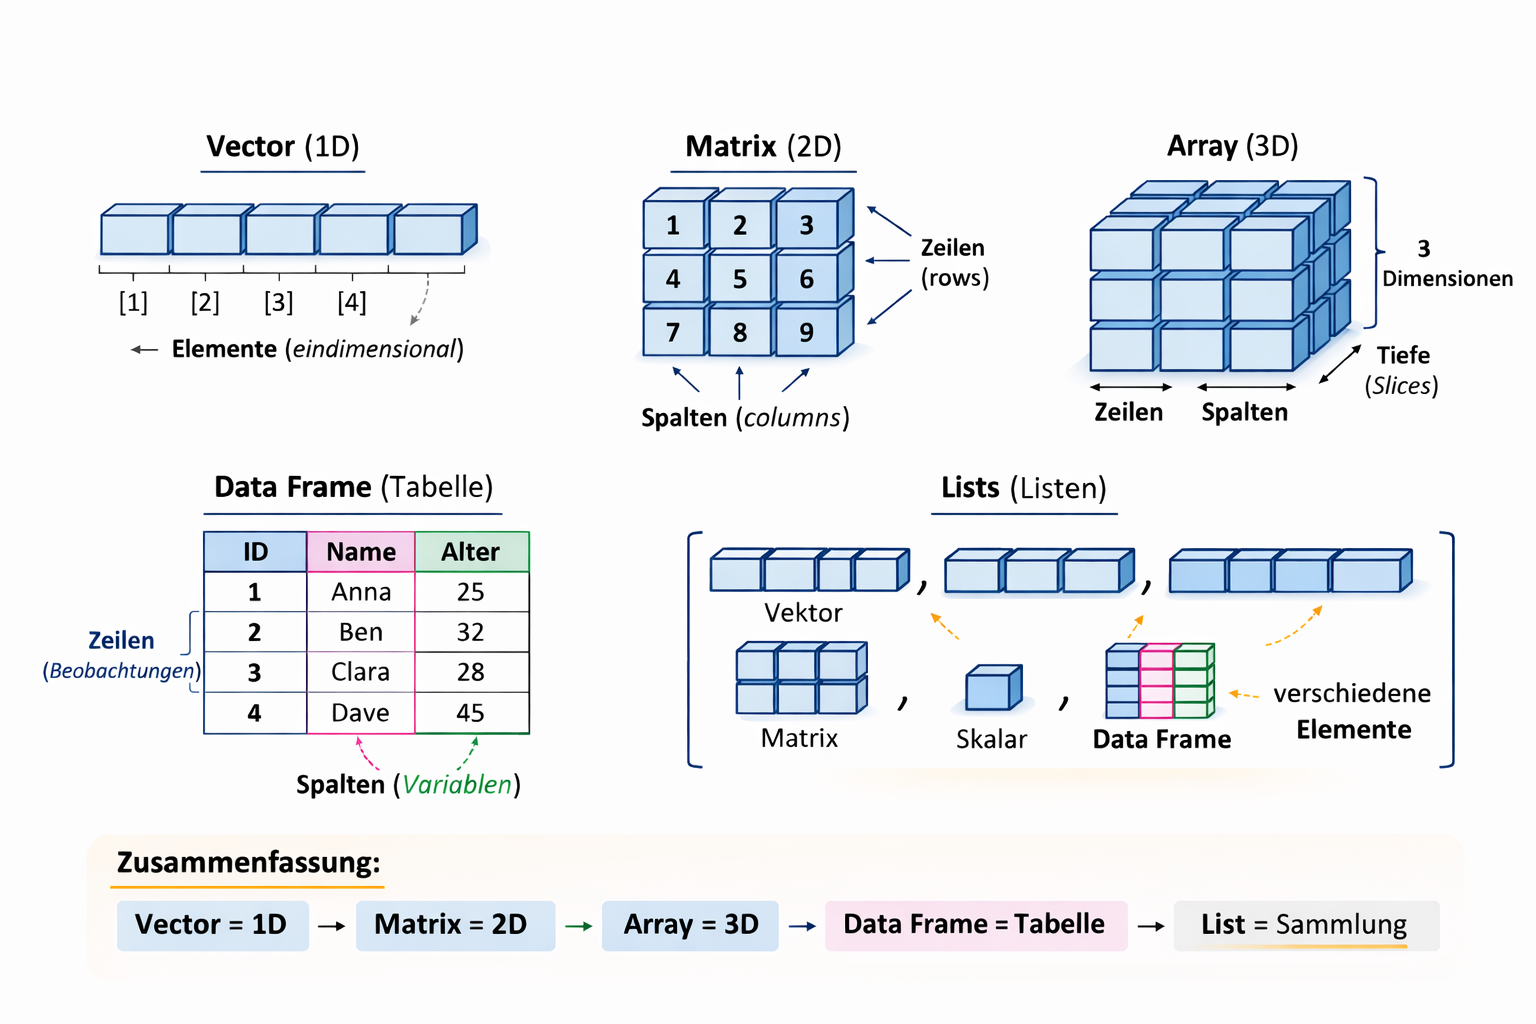
\includegraphics[keepaspectratio]{../figures/DataStructures.png}}

}

\caption{\label{fig-datastructure}Datenstrukturen in R, generiert mit
ChatGPT, angelehnt an
\href{https://bioinformatics-core-shared-training.github.io/Bitesize-R/week2.html}{R
for Biologists}}

\end{figure}%
\end{frame}

\begin{frame}{Big Picture: Welche Datenstruktur passt?}
\phantomsection\label{big-picture-welche-datenstruktur-passt}
\begin{longtable}[]{@{}lrll@{}}
\toprule\noalign{}
Struktur & Dimension & Datentypen & Typischer Einsatz \\
\midrule\noalign{}
\endhead
Vektor & 1D & einheitlich & Messwerte, Namen, logische Filter \\
Matrix & 2D & einheitlich & numerische Tabellen, lineare Algebra \\
Liste & flexibel & gemischt & Container für verschiedene Objekte \\
Data Frame & 2D & spaltenweise verschieden & Datensätze \\
Factor & 1D & Kategorien & Gruppen, Klassen, Bewertungen \\
\bottomrule\noalign{}
\end{longtable}
\end{frame}

\begin{frame}{Leitfrage}
\phantomsection\label{leitfrage}
\begin{quote}
Wie speichert R Daten so, dass wir damit rechnen, filtern und
analysieren können?
\end{quote}

Diskutieren Sie kurz zu zweit: 1. Was wäre eine passende Struktur für
Körpergrößen? 2. Was wäre eine passende Struktur für eine Tabelle mit
Alter, Geschlecht und Blutwerten? 3. Was wäre eine passende Struktur für
Antwortkategorien wie „niedrig``, „mittel``, „hoch``?
\end{frame}

\section{Vektoren}\label{vektoren}

\begin{frame}[fragile]{Vektoren: die zentrale Struktur}
\phantomsection\label{vektoren-die-zentrale-struktur}
Ein Vektor enthält mehrere Werte hintereinander.

\begin{Shaded}
\begin{Highlighting}[]
\NormalTok{x }\OtherTok{\textless{}{-}} \FunctionTok{c}\NormalTok{(}\FloatTok{1.7}\NormalTok{, }\FloatTok{3.8}\NormalTok{, }\FloatTok{4.2}\NormalTok{, }\FloatTok{5.7}\NormalTok{)}
\NormalTok{x}
\end{Highlighting}
\end{Shaded}

Wichtig:

\begin{itemize}
\tightlist
\item
  atomare Vektoren enthalten Werte \textbf{eines} Datentyps
\item
  viele R-Funktionen arbeiten automatisch elementweise
\item
  Vektoren sind Grundlage für viele andere Datenstrukturen
\end{itemize}
\end{frame}

\begin{frame}[fragile]{Vektoren erzeugen}
\phantomsection\label{vektoren-erzeugen}
\begin{Shaded}
\begin{Highlighting}[]
\FunctionTok{c}\NormalTok{(}\DecValTok{1}\NormalTok{, }\FloatTok{1.5}\NormalTok{, }\DecValTok{2}\NormalTok{)}

\FunctionTok{double}\NormalTok{(}\DecValTok{5}\NormalTok{)}

\DecValTok{1}\SpecialCharTok{:}\DecValTok{5}

\FunctionTok{rep}\NormalTok{(}\DecValTok{3}\NormalTok{, }\DecValTok{5}\NormalTok{)}

\FunctionTok{seq}\NormalTok{(}\DecValTok{0}\NormalTok{, }\FloatTok{0.6}\NormalTok{, }\AttributeTok{by =} \FloatTok{0.2}\NormalTok{)}
\end{Highlighting}
\end{Shaded}

\textbf{Mini-Frage:} Was ist der Unterschied zwischen \texttt{rep()} und
\texttt{seq()}?

\note{rep wiederholt Werte; seq erzeugt eine Zahlenfolge mit Start, Ende
und Schrittweite.}
\end{frame}

\begin{frame}[fragile]{Übung: Vektoren erzeugen}
\phantomsection\label{uxfcbung-vektoren-erzeugen}
Erzeugen Sie folgende Vektoren:

\begin{enumerate}
\tightlist
\item
  \texttt{2\ 4\ 6\ 8\ 10}
\item
  fünfmal den Wert \texttt{0}
\item
  die Zahlen von \texttt{0} bis \texttt{1} in Schritten von
  \texttt{0.25}
\item
  den Vektor \texttt{"ja"\ "nein"\ "ja"}
\end{enumerate}

\begin{Shaded}
\begin{Highlighting}[]
\CommentTok{\# Ihre Lösung}
\end{Highlighting}
\end{Shaded}
\end{frame}

\begin{frame}[fragile]{Indizierung: Zugriff auf Elemente}
\phantomsection\label{indizierung-zugriff-auf-elemente}
In R beginnt die Zählung bei \textbf{1}.

\begin{Shaded}
\begin{Highlighting}[]
\NormalTok{x }\OtherTok{\textless{}{-}} \FunctionTok{c}\NormalTok{(}\FloatTok{1.7}\NormalTok{, }\FloatTok{3.8}\NormalTok{, }\FloatTok{4.2}\NormalTok{, }\FloatTok{5.7}\NormalTok{)}

\NormalTok{x[}\DecValTok{2}\NormalTok{]}
\NormalTok{x[}\DecValTok{2}\SpecialCharTok{:}\DecValTok{3}\NormalTok{]}
\NormalTok{x[}\FunctionTok{c}\NormalTok{(}\DecValTok{4}\NormalTok{, }\DecValTok{4}\NormalTok{, }\DecValTok{1}\NormalTok{)]}
\NormalTok{x[}\SpecialCharTok{{-}}\FunctionTok{c}\NormalTok{(}\DecValTok{1}\NormalTok{, }\DecValTok{2}\NormalTok{)]}
\end{Highlighting}
\end{Shaded}

Merksatz:

\begin{itemize}
\tightlist
\item
  \texttt{x{[}i{]}}: einzelnes Element
\item
  \texttt{x{[}i:j{]}}: zusammenhängender Bereich
\item
  \texttt{x{[}c(...){]}}: beliebige Auswahl
\item
  \texttt{x{[}-i{]}}: Element ausschließen
\end{itemize}
\end{frame}

\begin{frame}[fragile]{Logische Indizierung}
\phantomsection\label{logische-indizierung}
Ein logischer Vektor wirkt wie ein Filter.

\begin{Shaded}
\begin{Highlighting}[]
\NormalTok{x }\OtherTok{\textless{}{-}} \FunctionTok{c}\NormalTok{(}\FloatTok{1.7}\NormalTok{, }\FloatTok{0.5}\NormalTok{, }\SpecialCharTok{{-}}\FloatTok{0.7}\NormalTok{, }\DecValTok{0}\NormalTok{, }\FloatTok{2.8}\NormalTok{, }\FloatTok{0.2}\NormalTok{)}

\NormalTok{x[}\FunctionTok{c}\NormalTok{(}\ConstantTok{TRUE}\NormalTok{, }\ConstantTok{TRUE}\NormalTok{, }\ConstantTok{FALSE}\NormalTok{, }\ConstantTok{FALSE}\NormalTok{, }\ConstantTok{TRUE}\NormalTok{, }\ConstantTok{TRUE}\NormalTok{)]}
\end{Highlighting}
\end{Shaded}

\texttt{TRUE} lässt ein Element passieren, \texttt{FALSE} entfernt es.
\end{frame}

\begin{frame}[fragile]{Filtern mit Bedingungen}
\phantomsection\label{filtern-mit-bedingungen}
\begin{Shaded}
\begin{Highlighting}[]
\NormalTok{x }\OtherTok{\textless{}{-}} \FunctionTok{c}\NormalTok{(}\FloatTok{0.3}\NormalTok{, }\FloatTok{0.1}\NormalTok{, }\FloatTok{5.7}\NormalTok{, }\SpecialCharTok{{-}}\FloatTok{1.0}\NormalTok{)}

\NormalTok{x }\SpecialCharTok{\textgreater{}} \DecValTok{0}

\NormalTok{x[x }\SpecialCharTok{\textgreater{}} \DecValTok{0}\NormalTok{]}
\end{Highlighting}
\end{Shaded}

Eine Bedingung erzeugt zuerst einen logischen Vektor.

Dieser logische Vektor wird dann als Index benutzt.
\end{frame}

\begin{frame}[fragile]{Positionen finden mit \texttt{which()}}
\phantomsection\label{positionen-finden-mit-which}
Manchmal interessieren nicht die Werte, sondern die Positionen.

\begin{Shaded}
\begin{Highlighting}[]
\NormalTok{x }\OtherTok{\textless{}{-}} \FunctionTok{c}\NormalTok{(}\FloatTok{0.3}\NormalTok{, }\FloatTok{0.1}\NormalTok{, }\FloatTok{5.7}\NormalTok{, }\SpecialCharTok{{-}}\FloatTok{1.0}\NormalTok{)}

\FunctionTok{which}\NormalTok{(x }\SpecialCharTok{\textgreater{}} \DecValTok{0}\NormalTok{)}
\end{Highlighting}
\end{Shaded}

\texttt{which()} gibt die Positionen zurück, an denen eine Bedingung
\texttt{TRUE} ist.
\end{frame}

\begin{frame}[fragile]{Vektoren kombinieren}
\phantomsection\label{vektoren-kombinieren}
\begin{Shaded}
\begin{Highlighting}[]
\NormalTok{x }\OtherTok{\textless{}{-}} \FunctionTok{c}\NormalTok{(}\FloatTok{0.3}\NormalTok{, }\FloatTok{0.1}\NormalTok{, }\FloatTok{5.7}\NormalTok{, }\SpecialCharTok{{-}}\FloatTok{1.0}\NormalTok{)}
\NormalTok{y }\OtherTok{\textless{}{-}} \FunctionTok{c}\NormalTok{(}\DecValTok{2}\NormalTok{, }\DecValTok{3}\NormalTok{, }\DecValTok{1}\NormalTok{, }\DecValTok{5}\NormalTok{)}

\FunctionTok{c}\NormalTok{(x, y)}
\end{Highlighting}
\end{Shaded}

\texttt{c()} steht für \textbf{combine}.
\end{frame}

\begin{frame}[fragile]{Skalare Operationen}
\phantomsection\label{skalare-operationen}
R rechnet elementweise.

\begin{Shaded}
\begin{Highlighting}[]
\NormalTok{x }\OtherTok{\textless{}{-}} \FunctionTok{c}\NormalTok{(}\DecValTok{1}\NormalTok{, }\FloatTok{1.5}\NormalTok{, }\DecValTok{2}\NormalTok{)}

\NormalTok{x }\SpecialCharTok{+} \DecValTok{2}
\NormalTok{x }\SpecialCharTok{{-}} \DecValTok{2}
\NormalTok{x }\SpecialCharTok{*} \DecValTok{2}
\NormalTok{x }\SpecialCharTok{/} \DecValTok{2}
\end{Highlighting}
\end{Shaded}

Jedes Element wird einzeln verarbeitet.
\end{frame}

\begin{frame}[fragile]{Vektor-Arithmetik}
\phantomsection\label{vektor-arithmetik}
Bei gleich langen Vektoren werden Elemente paarweise verrechnet.

\begin{Shaded}
\begin{Highlighting}[]
\FunctionTok{c}\NormalTok{(}\DecValTok{1}\NormalTok{, }\DecValTok{2}\NormalTok{, }\DecValTok{3}\NormalTok{) }\SpecialCharTok{+} \FunctionTok{c}\NormalTok{(}\FloatTok{1.2}\NormalTok{, }\SpecialCharTok{{-}}\FloatTok{0.5}\NormalTok{, }\SpecialCharTok{{-}}\FloatTok{0.1}\NormalTok{)}

\FunctionTok{c}\NormalTok{(}\DecValTok{1}\NormalTok{, }\DecValTok{2}\NormalTok{, }\DecValTok{3}\NormalTok{) }\SpecialCharTok{*} \FunctionTok{c}\NormalTok{(}\FloatTok{1.2}\NormalTok{, }\SpecialCharTok{{-}}\FloatTok{0.5}\NormalTok{, }\SpecialCharTok{{-}}\FloatTok{0.1}\NormalTok{)}
\end{Highlighting}
\end{Shaded}
\end{frame}

\begin{frame}[fragile]{Recycling-Prinzip}
\phantomsection\label{recycling-prinzip}
Wenn Vektoren unterschiedlich lang sind, wiederholt R den kürzeren
Vektor.

\begin{Shaded}
\begin{Highlighting}[]
\FunctionTok{c}\NormalTok{(}\DecValTok{1}\NormalTok{, }\DecValTok{1}\NormalTok{, }\DecValTok{1}\NormalTok{, }\DecValTok{1}\NormalTok{, }\DecValTok{1}\NormalTok{) }\SpecialCharTok{*} \FunctionTok{c}\NormalTok{(}\DecValTok{1}\NormalTok{, }\DecValTok{2}\NormalTok{, }\DecValTok{3}\NormalTok{)}
\end{Highlighting}
\end{Shaded}

R interpretiert dies intern ungefähr als:

\begin{Shaded}
\begin{Highlighting}[]
\FunctionTok{c}\NormalTok{(}\DecValTok{1}\NormalTok{, }\DecValTok{1}\NormalTok{, }\DecValTok{1}\NormalTok{, }\DecValTok{1}\NormalTok{, }\DecValTok{1}\NormalTok{) }\SpecialCharTok{*} \FunctionTok{c}\NormalTok{(}\DecValTok{1}\NormalTok{, }\DecValTok{2}\NormalTok{, }\DecValTok{3}\NormalTok{, }\DecValTok{1}\NormalTok{, }\DecValTok{2}\NormalTok{)}
\end{Highlighting}
\end{Shaded}

Achten Sie auf Warnungen, wenn die Längen nicht gut zusammenpassen.
\end{frame}

\begin{frame}[fragile]{Funktionen auf Vektoren}
\phantomsection\label{funktionen-auf-vektoren}
Viele Funktionen arbeiten elementweise:

\begin{Shaded}
\begin{Highlighting}[]
\FunctionTok{exp}\NormalTok{(}\FunctionTok{c}\NormalTok{(}\DecValTok{0}\NormalTok{, }\DecValTok{1}\NormalTok{, }\DecValTok{2}\NormalTok{, }\DecValTok{3}\NormalTok{))}
\FunctionTok{sqrt}\NormalTok{(}\FunctionTok{c}\NormalTok{(}\DecValTok{4}\NormalTok{, }\DecValTok{9}\NormalTok{, }\DecValTok{16}\NormalTok{))}
\end{Highlighting}
\end{Shaded}

Andere Funktionen fassen einen Vektor zu einem Wert zusammen:

\begin{Shaded}
\begin{Highlighting}[]
\FunctionTok{mean}\NormalTok{(}\FunctionTok{c}\NormalTok{(}\FloatTok{1.2}\NormalTok{, }\SpecialCharTok{{-}}\FloatTok{0.5}\NormalTok{, }\SpecialCharTok{{-}}\FloatTok{0.1}\NormalTok{))}
\FunctionTok{sum}\NormalTok{(}\FunctionTok{c}\NormalTok{(}\DecValTok{1}\NormalTok{, }\DecValTok{2}\NormalTok{, }\DecValTok{3}\NormalTok{))}
\FunctionTok{length}\NormalTok{(}\FunctionTok{c}\NormalTok{(}\DecValTok{1}\NormalTok{, }\DecValTok{2}\NormalTok{, }\DecValTok{3}\NormalTok{))}
\end{Highlighting}
\end{Shaded}
\end{frame}

\begin{frame}[fragile]{Skalarprodukt}
\phantomsection\label{skalarprodukt}
\begin{Shaded}
\begin{Highlighting}[]
\NormalTok{a }\OtherTok{\textless{}{-}} \FunctionTok{c}\NormalTok{(}\DecValTok{1}\NormalTok{, }\DecValTok{2}\NormalTok{, }\DecValTok{3}\NormalTok{)}
\NormalTok{b }\OtherTok{\textless{}{-}} \FunctionTok{c}\NormalTok{(}\FloatTok{1.2}\NormalTok{, }\SpecialCharTok{{-}}\FloatTok{0.5}\NormalTok{, }\SpecialCharTok{{-}}\FloatTok{0.1}\NormalTok{)}

\NormalTok{a }\SpecialCharTok{\%*\%}\NormalTok{ b}
\end{Highlighting}
\end{Shaded}

Das Skalarprodukt multipliziert paarweise und summiert anschließend.
\end{frame}

\begin{frame}[fragile]{Aktivierung: CRP-Werte}
\phantomsection\label{aktivierung-crp-werte}
\begin{Shaded}
\begin{Highlighting}[]
\NormalTok{crp }\OtherTok{\textless{}{-}} \FunctionTok{c}\NormalTok{(}\FloatTok{2.1}\NormalTok{, }\FloatTok{8.4}\NormalTok{, }\FloatTok{0.6}\NormalTok{, }\FloatTok{12.3}\NormalTok{, }\FloatTok{3.2}\NormalTok{, }\FloatTok{15.7}\NormalTok{, }\FloatTok{1.0}\NormalTok{)}
\end{Highlighting}
\end{Shaded}

Aufgaben:

\begin{enumerate}
\tightlist
\item
  Welche Werte sind größer als \texttt{5}?
\item
  Filtern Sie alle Werte über \texttt{5}.
\item
  Bestimmen Sie die Positionen dieser Werte.
\item
  Ergänzen Sie \texttt{crp\_neu\ \textless{}-\ c(4.3,\ 9.8)}.
\end{enumerate}

\begin{Shaded}
\begin{Highlighting}[]
\CommentTok{\# Ihre Lösung}
\end{Highlighting}
\end{Shaded}
\end{frame}

\section{Matrizen}\label{matrizen}

\begin{frame}{Was ist eine Matrix?}
\phantomsection\label{was-ist-eine-matrix}
Eine Matrix ist ein zweidimensionaler Container.

Eigenschaften:

\begin{itemize}
\tightlist
\item
  Zeilen × Spalten
\item
  alle Elemente haben denselben Datentyp
\item
  nützlich für numerische Berechnungen und lineare Algebra
\end{itemize}
\end{frame}

\begin{frame}[fragile]{Matrix erzeugen}
\phantomsection\label{matrix-erzeugen}
\begin{Shaded}
\begin{Highlighting}[]
\NormalTok{x }\OtherTok{\textless{}{-}} \FunctionTok{matrix}\NormalTok{(}\DecValTok{1}\SpecialCharTok{:}\DecValTok{6}\NormalTok{, }\AttributeTok{nrow =} \DecValTok{2}\NormalTok{, }\AttributeTok{ncol =} \DecValTok{3}\NormalTok{)}
\NormalTok{x}
\end{Highlighting}
\end{Shaded}

\begin{verbatim}
     [,1] [,2] [,3]
[1,]    1    3    5
[2,]    2    4    6
\end{verbatim}

Wichtig:

R füllt Matrizen standardmäßig \textbf{spaltenweise}.
\end{frame}

\begin{frame}[fragile]{Matrix-Indizierung}
\phantomsection\label{matrix-indizierung}
Allgemeine Form:

\begin{Shaded}
\begin{Highlighting}[]
\NormalTok{x[Zeile, Spalte]}
\end{Highlighting}
\end{Shaded}
\end{frame}

\begin{frame}[fragile]{Matrix-Indizierung}
\phantomsection\label{matrix-indizierung-1}
Beispiele:

\begin{Shaded}
\begin{Highlighting}[]
\NormalTok{x[}\DecValTok{1}\NormalTok{, }\DecValTok{3}\NormalTok{]    }\CommentTok{\# einzelnes Element}
\end{Highlighting}
\end{Shaded}

\begin{verbatim}
[1] 5
\end{verbatim}

\begin{Shaded}
\begin{Highlighting}[]
\NormalTok{x[}\DecValTok{2}\NormalTok{, ]     }\CommentTok{\# ganze Zeile}
\end{Highlighting}
\end{Shaded}

\begin{verbatim}
[1] 2 4 6
\end{verbatim}

\begin{Shaded}
\begin{Highlighting}[]
\NormalTok{x[, }\DecValTok{2}\NormalTok{]     }\CommentTok{\# ganze Spalte}
\end{Highlighting}
\end{Shaded}

\begin{verbatim}
[1] 3 4
\end{verbatim}

\begin{Shaded}
\begin{Highlighting}[]
\NormalTok{x[, }\DecValTok{1}\SpecialCharTok{:}\DecValTok{2}\NormalTok{]   }\CommentTok{\# mehrere Spalten}
\end{Highlighting}
\end{Shaded}

\begin{verbatim}
     [,1] [,2]
[1,]    1    3
[2,]    2    4
\end{verbatim}
\end{frame}

\begin{frame}[fragile]{\texttt{drop\ =\ FALSE}}
\phantomsection\label{drop-false}
\begin{Shaded}
\begin{Highlighting}[]
\NormalTok{x[}\DecValTok{2}\NormalTok{, , drop }\OtherTok{=} \ConstantTok{FALSE}\NormalTok{]}
\end{Highlighting}
\end{Shaded}

\begin{verbatim}
     [,1] [,2] [,3]
[1,]    2    4    6
\end{verbatim}

\begin{Shaded}
\begin{Highlighting}[]
\NormalTok{x[, }\DecValTok{2}\NormalTok{, drop }\OtherTok{=} \ConstantTok{FALSE}\NormalTok{]}
\end{Highlighting}
\end{Shaded}

\begin{verbatim}
     [,1]
[1,]    3
[2,]    4
\end{verbatim}

Ohne \texttt{drop\ =\ FALSE} macht R aus einer einzelnen Zeile oder
Spalte oft einen Vektor.

Mit \texttt{drop\ =\ FALSE} bleibt die Matrixstruktur erhalten.
\end{frame}

\begin{frame}[fragile]{Lineare Indizierung}
\phantomsection\label{lineare-indizierung}
Matrizen können auch wie ein Vektor indiziert werden.

\begin{Shaded}
\begin{Highlighting}[]
\NormalTok{x }\OtherTok{\textless{}{-}} \FunctionTok{matrix}\NormalTok{(}\FunctionTok{c}\NormalTok{(}\DecValTok{10}\NormalTok{, }\DecValTok{50}\NormalTok{, }\DecValTok{3}\NormalTok{, }\DecValTok{99}\NormalTok{, }\SpecialCharTok{{-}}\DecValTok{1}\NormalTok{, }\DecValTok{8}\NormalTok{), }\AttributeTok{nrow =} \DecValTok{2}\NormalTok{)}
\NormalTok{x}
\end{Highlighting}
\end{Shaded}

\begin{verbatim}
     [,1] [,2] [,3]
[1,]   10    3   -1
[2,]   50   99    8
\end{verbatim}

\begin{Shaded}
\begin{Highlighting}[]
\NormalTok{x[}\DecValTok{1}\NormalTok{]}
\end{Highlighting}
\end{Shaded}

\begin{verbatim}
[1] 10
\end{verbatim}

\begin{Shaded}
\begin{Highlighting}[]
\NormalTok{x[}\DecValTok{5}\NormalTok{]}
\end{Highlighting}
\end{Shaded}

\begin{verbatim}
[1] -1
\end{verbatim}

Bei x{[}\ldots{]} ohne Komma wird keine Zeilen- und Spaltenstruktur mehr
verwendet. R behandelt die Matrix dann wie einen langen Vektor. Deshalb
nennt man das lineare Indizierung.
\end{frame}

\begin{frame}[fragile]{Lineare Indizierung}
\phantomsection\label{lineare-indizierung-1}
\begin{Shaded}
\begin{Highlighting}[]
\NormalTok{x[x }\SpecialCharTok{\textless{}} \DecValTok{3}\NormalTok{]}
\end{Highlighting}
\end{Shaded}

\begin{verbatim}
[1] -1
\end{verbatim}

R prüft jedes Element der Matrix:

\begin{verbatim}
      [,1]  [,2]  [,3]
[1,] FALSE FALSE  TRUE
[2,] FALSE FALSE FALSE
\end{verbatim}

Nur Elemente mit \texttt{TRUE} werden ausgewählt.

Das Ergebnis ist ein Vektor, keine Matrix.
\end{frame}

\begin{frame}[fragile]{Zeilen- und Spaltennamen}
\phantomsection\label{zeilen--und-spaltennamen}
\begin{Shaded}
\begin{Highlighting}[]
\FunctionTok{colnames}\NormalTok{(x) }\OtherTok{\textless{}{-}} \FunctionTok{c}\NormalTok{(}\StringTok{"C1"}\NormalTok{, }\StringTok{"C2"}\NormalTok{, }\StringTok{"C3"}\NormalTok{)}
\FunctionTok{rownames}\NormalTok{(x) }\OtherTok{\textless{}{-}} \FunctionTok{c}\NormalTok{(}\StringTok{"R1"}\NormalTok{, }\StringTok{"R2"}\NormalTok{)}

\NormalTok{x}
\end{Highlighting}
\end{Shaded}

\begin{verbatim}
   C1 C2 C3
R1 10  3 -1
R2 50 99  8
\end{verbatim}

Namen machen Code lesbarer.
\end{frame}

\begin{frame}[fragile]{Mini-Übung: Matrix}
\phantomsection\label{mini-uxfcbung-matrix}
\begin{Shaded}
\begin{Highlighting}[]
\NormalTok{m }\OtherTok{\textless{}{-}} \FunctionTok{matrix}\NormalTok{(}\DecValTok{1}\SpecialCharTok{:}\DecValTok{12}\NormalTok{, }\AttributeTok{nrow =} \DecValTok{3}\NormalTok{)}
\end{Highlighting}
\end{Shaded}

Aufgaben:

\begin{enumerate}
\tightlist
\item
  Geben Sie die zweite Zeile aus.
\item
  Geben Sie die dritte Spalte aus.
\item
  Geben Sie das Element in Zeile 3, Spalte 2 aus.
\item
  Benennen Sie die Spalten mit \texttt{A}, \texttt{B}, \texttt{C},
  \texttt{D}.
\item
  Geben Sie nur die Spalte \texttt{A} und \texttt{C} aus.
\item
  Schließen Sie die zweite Zeile aus.
\item
  Geben Sie die Positionen aller Werte größer als 10 mit Zeilen- und
  Spaltenangabe aus.
\end{enumerate}
\end{frame}

\begin{frame}[fragile]{Matrix-Funktionen (1/3)}
\phantomsection\label{matrix-funktionen-13}
Eine Matrix erzeugen:

\begin{verbatim}
     [,1] [,2] [,3]
[1,]    1    3    5
[2,]    2    4    6
\end{verbatim}

Dimensionen abfragen:

\begin{Shaded}
\begin{Highlighting}[]
\FunctionTok{dim}\NormalTok{(A)     }\CommentTok{\# Zeilen und Spalten}
\end{Highlighting}
\end{Shaded}

\begin{verbatim}
[1] 2 3
\end{verbatim}

\begin{Shaded}
\begin{Highlighting}[]
\FunctionTok{nrow}\NormalTok{(A)   }\CommentTok{\# Anzahl Zeilen}
\end{Highlighting}
\end{Shaded}

\begin{verbatim}
[1] 2
\end{verbatim}

\begin{Shaded}
\begin{Highlighting}[]
\FunctionTok{ncol}\NormalTok{(A)   }\CommentTok{\# Anzahl Spalten}
\end{Highlighting}
\end{Shaded}

\begin{verbatim}
[1] 3
\end{verbatim}
\end{frame}

\begin{frame}[fragile]{Matrix-Funktionen (2/3)}
\phantomsection\label{matrix-funktionen-23}
Anzahl Elemente abfragen:

\begin{Shaded}
\begin{Highlighting}[]
\FunctionTok{length}\NormalTok{(A) }\CommentTok{\# Anzahl gespeicherter Werte}
\end{Highlighting}
\end{Shaded}

\begin{verbatim}
[1] 6
\end{verbatim}

Wichtig: \texttt{length(A)} zählt \textbf{alle Elemente}, nicht die
Anzahl der Zeilen.
\end{frame}

\begin{frame}[fragile]{Matrix-Funktionen (3/3)}
\phantomsection\label{matrix-funktionen-33}
Transponieren einer Matrix:

\begin{Shaded}
\begin{Highlighting}[]
\NormalTok{A }\OtherTok{\textless{}{-}} \FunctionTok{matrix}\NormalTok{(}\DecValTok{1}\SpecialCharTok{:}\DecValTok{6}\NormalTok{, }\AttributeTok{nrow =} \DecValTok{2}\NormalTok{, }\AttributeTok{ncol =} \DecValTok{3}\NormalTok{)}
\NormalTok{A}
\end{Highlighting}
\end{Shaded}

\begin{verbatim}
     [,1] [,2] [,3]
[1,]    1    3    5
[2,]    2    4    6
\end{verbatim}

\begin{Shaded}
\begin{Highlighting}[]
\FunctionTok{t}\NormalTok{(A)}
\end{Highlighting}
\end{Shaded}

\begin{verbatim}
     [,1] [,2]
[1,]    1    2
[2,]    3    4
[3,]    5    6
\end{verbatim}

\texttt{t(A)} vertauscht Zeilen und Spalten.
\end{frame}

\begin{frame}[fragile]{Matrixmultiplikation}
\phantomsection\label{matrixmultiplikation}
\begin{columns}[T]
\begin{column}{0.5\linewidth}
Matrix \texttt{A}:

\begin{Shaded}
\begin{Highlighting}[]
\NormalTok{A }\OtherTok{\textless{}{-}} \FunctionTok{matrix}\NormalTok{(}\DecValTok{1}\SpecialCharTok{:}\DecValTok{6}\NormalTok{, }\AttributeTok{nrow =} \DecValTok{2}\NormalTok{, }\AttributeTok{ncol =} \DecValTok{3}\NormalTok{)}
\NormalTok{A}
\end{Highlighting}
\end{Shaded}

\begin{verbatim}
     [,1] [,2] [,3]
[1,]    1    3    5
[2,]    2    4    6
\end{verbatim}
\end{column}

\begin{column}{0.5\linewidth}
Matrix \texttt{B}:

\begin{Shaded}
\begin{Highlighting}[]
\NormalTok{B }\OtherTok{\textless{}{-}} \FunctionTok{matrix}\NormalTok{(}\DecValTok{1}\SpecialCharTok{:}\DecValTok{6}\NormalTok{, }\AttributeTok{nrow =} \DecValTok{3}\NormalTok{, }\AttributeTok{ncol =} \DecValTok{2}\NormalTok{)}
\NormalTok{B}
\end{Highlighting}
\end{Shaded}

\begin{verbatim}
     [,1] [,2]
[1,]    1    4
[2,]    2    5
[3,]    3    6
\end{verbatim}
\end{column}
\end{columns}

\begin{Shaded}
\begin{Highlighting}[]
\NormalTok{A }\SpecialCharTok{\%*\%}\NormalTok{ B}
\end{Highlighting}
\end{Shaded}

\begin{verbatim}
     [,1] [,2]
[1,]   22   49
[2,]   28   64
\end{verbatim}

Wichtig: Für \texttt{A\ \%*\%\ B} muss die Anzahl der Spalten von
\texttt{A} zur Anzahl der Zeilen von \texttt{B} passen.
\end{frame}

\section{Listen}\label{listen}

\begin{frame}[fragile]{Listen: flexible Container}
\phantomsection\label{listen-flexible-container}
Listen können verschiedene Objekte enthalten.

\begin{Shaded}
\begin{Highlighting}[]
\NormalTok{L }\OtherTok{\textless{}{-}} \FunctionTok{list}\NormalTok{(}\AttributeTok{servus=}\StringTok{"hallo"}\NormalTok{, }\FunctionTok{c}\NormalTok{(}\DecValTok{1}\NormalTok{, }\DecValTok{3}\NormalTok{, }\DecValTok{7}\NormalTok{), }\FunctionTok{matrix}\NormalTok{(}\DecValTok{1}\SpecialCharTok{:}\DecValTok{6}\NormalTok{, }\DecValTok{3}\NormalTok{))}
\NormalTok{L}
\end{Highlighting}
\end{Shaded}

\begin{verbatim}
$servus
[1] "hallo"

[[2]]
[1] 1 3 7

[[3]]
     [,1] [,2]
[1,]    1    4
[2,]    2    5
[3,]    3    6
\end{verbatim}

Eine Liste kann also Text, Vektoren, Matrizen oder weitere Listen
enthalten.
\end{frame}

\begin{frame}[fragile]{Listen indizieren: \texttt{{[}\ {]}}
vs.~\texttt{{[}{[}\ {]}{]}}}
\phantomsection\label{listen-indizieren-vs.}
Mit \texttt{{[}\ {]}} erhält man eine Teilliste:

\begin{Shaded}
\begin{Highlighting}[]
\NormalTok{L[}\DecValTok{1}\NormalTok{]}
\end{Highlighting}
\end{Shaded}

\begin{verbatim}
$servus
[1] "hallo"
\end{verbatim}

Mit \texttt{{[}{[}\ {]}{]}} erhält man das gespeicherte Element selbst:

\begin{Shaded}
\begin{Highlighting}[]
\NormalTok{L[[}\DecValTok{1}\NormalTok{]]}
\end{Highlighting}
\end{Shaded}

\begin{verbatim}
[1] "hallo"
\end{verbatim}

Merke:

\begin{itemize}
\tightlist
\item
  \texttt{L{[}i{]}} gibt eine Liste zurück
\item
  \texttt{L{[}{[}i{]}{]}} gibt das Element zurück
\end{itemize}
\end{frame}

\begin{frame}[fragile]{Zugriff auf Listen}
\phantomsection\label{zugriff-auf-listen}
\texttt{L\$name} greift auf ein benanntes Element zu

\begin{Shaded}
\begin{Highlighting}[]
\NormalTok{L}\SpecialCharTok{$}\NormalTok{servus}
\end{Highlighting}
\end{Shaded}

\begin{verbatim}
[1] "hallo"
\end{verbatim}
\end{frame}

\begin{frame}[fragile]{Mini-Übung: Listen}
\phantomsection\label{mini-uxfcbung-listen}
Erstellen Sie eine Liste \texttt{person} mit:

\begin{itemize}
\tightlist
\item
  Name
\item
  Alter
\item
  Lieblingszahlen als Vektor
\item
  einer logischen Angabe \texttt{student}
\end{itemize}

1. Geben Sie nur den Namen aus.\\
2. Geben Sie nur die Lieblingszahlen aus.\\
3. Geben Sie die zweite Lieblingszahl aus.\\
4. Prüfen Sie, ob die Person Studentin oder Student ist.\\
5. Geben Sie alle Lieblingszahlen aus, die größer als 5 sind.\\
6. Ergänzen Sie die Liste um den Wohnort ``Ingolstadt''.\\
7. Löschen Sie das Element alter.
\end{frame}

\begin{frame}{Listen: Zusammenfassung}
\phantomsection\label{listen-zusammenfassung}
Listen sind flexible Container für Objekte, die zusammengehören, aber
unterschiedlich aufgebaut sein können.

Viele R-Objekte sind intern Listen, zum Beispiel Modelle oder Data
Frames.
\end{frame}

\section{Data Frames}\label{data-frames}

\begin{frame}{Data Frames}
\phantomsection\label{data-frames-1}
Ein Data Frame ist die zentrale Struktur für tabellarische Daten.

Eigenschaften:

\begin{itemize}
\tightlist
\item
  zweidimensional: Zeilen und Spalten
\item
  jede Spalte ist ein Vektor
\item
  Spalten dürfen unterschiedliche Datentypen haben
\item
  innerhalb einer Spalte ist der Datentyp einheitlich
\end{itemize}
\end{frame}

\begin{frame}[fragile]{Data Frame erstellen}
\phantomsection\label{data-frame-erstellen}
\begin{Shaded}
\begin{Highlighting}[]
\NormalTok{df }\OtherTok{\textless{}{-}} \FunctionTok{data.frame}\NormalTok{(}
  \AttributeTok{foo =} \DecValTok{1}\SpecialCharTok{:}\DecValTok{4}\NormalTok{,}
  \AttributeTok{bar =} \FunctionTok{c}\NormalTok{(}\ConstantTok{TRUE}\NormalTok{, }\ConstantTok{TRUE}\NormalTok{, }\ConstantTok{FALSE}\NormalTok{, }\ConstantTok{FALSE}\NormalTok{)}
\NormalTok{)}

\NormalTok{df}
\end{Highlighting}
\end{Shaded}

\begin{verbatim}
  foo   bar
1   1  TRUE
2   2  TRUE
3   3 FALSE
4   4 FALSE
\end{verbatim}

\begin{Shaded}
\begin{Highlighting}[]
\FunctionTok{nrow}\NormalTok{(df)}
\end{Highlighting}
\end{Shaded}

\begin{verbatim}
[1] 4
\end{verbatim}

\begin{Shaded}
\begin{Highlighting}[]
\FunctionTok{ncol}\NormalTok{(df)}
\end{Highlighting}
\end{Shaded}

\begin{verbatim}
[1] 2
\end{verbatim}
\end{frame}

\begin{frame}[fragile]{Datensatz \texttt{iris}}
\phantomsection\label{datensatz-iris}
\begin{Shaded}
\begin{Highlighting}[]
\FunctionTok{data}\NormalTok{(iris)}

\NormalTok{U }\OtherTok{\textless{}{-}}\NormalTok{ iris[}\FunctionTok{c}\NormalTok{(}\DecValTok{1}\NormalTok{, }\DecValTok{51}\NormalTok{, }\DecValTok{101}\NormalTok{), ]}
\NormalTok{U}
\end{Highlighting}
\end{Shaded}

\begin{verbatim}
    Sepal.Length Sepal.Width Petal.Length Petal.Width    Species
1            5.1         3.5          1.4         0.2     setosa
51           7.0         3.2          4.7         1.4 versicolor
101          6.3         3.3          6.0         2.5  virginica
\end{verbatim}

\texttt{iris} ist ein eingebauter Beispieldatensatz.
\end{frame}

\begin{frame}[fragile]{Indizierung von Data Frames}
\phantomsection\label{indizierung-von-data-frames}
\begin{Shaded}
\begin{Highlighting}[]
\NormalTok{U[}\DecValTok{1}\NormalTok{, ]}
\end{Highlighting}
\end{Shaded}

\begin{verbatim}
  Sepal.Length Sepal.Width Petal.Length Petal.Width Species
1          5.1         3.5          1.4         0.2  setosa
\end{verbatim}

\begin{Shaded}
\begin{Highlighting}[]
\NormalTok{U[, }\DecValTok{1}\NormalTok{]}
\end{Highlighting}
\end{Shaded}

\begin{verbatim}
[1] 5.1 7.0 6.3
\end{verbatim}

\begin{Shaded}
\begin{Highlighting}[]
\NormalTok{U}\SpecialCharTok{$}\NormalTok{Sepal.Length}
\end{Highlighting}
\end{Shaded}

\begin{verbatim}
[1] 5.1 7.0 6.3
\end{verbatim}

\begin{Shaded}
\begin{Highlighting}[]
\NormalTok{U[, }\FunctionTok{c}\NormalTok{(}\DecValTok{1}\NormalTok{, }\DecValTok{3}\NormalTok{)]}
\end{Highlighting}
\end{Shaded}

\begin{verbatim}
    Sepal.Length Petal.Length
1            5.1          1.4
51           7.0          4.7
101          6.3          6.0
\end{verbatim}
\end{frame}

\begin{frame}[fragile]{Filtern von Zeilen}
\phantomsection\label{filtern-von-zeilen}
\begin{Shaded}
\begin{Highlighting}[]
\NormalTok{U[U}\SpecialCharTok{$}\NormalTok{Sepal.Length }\SpecialCharTok{\textgreater{}} \DecValTok{5}\NormalTok{, ]}
\end{Highlighting}
\end{Shaded}

\begin{verbatim}
    Sepal.Length Sepal.Width Petal.Length Petal.Width    Species
1            5.1         3.5          1.4         0.2     setosa
51           7.0         3.2          4.7         1.4 versicolor
101          6.3         3.3          6.0         2.5  virginica
\end{verbatim}

Die Bedingung erzeugt einen logischen Vektor.

Nur Zeilen mit \texttt{TRUE} werden ausgewählt.
\end{frame}

\begin{frame}[fragile]{Ausschließen mit \texttt{-} und \texttt{!}}
\phantomsection\label{ausschlieuxdfen-mit---und}
\begin{Shaded}
\begin{Highlighting}[]
\NormalTok{U[}\SpecialCharTok{{-}}\DecValTok{1}\NormalTok{, ]}
\end{Highlighting}
\end{Shaded}

\begin{verbatim}
    Sepal.Length Sepal.Width Petal.Length Petal.Width    Species
51           7.0         3.2          4.7         1.4 versicolor
101          6.3         3.3          6.0         2.5  virginica
\end{verbatim}

\begin{Shaded}
\begin{Highlighting}[]
\NormalTok{U[}\SpecialCharTok{!}\NormalTok{(U}\SpecialCharTok{$}\NormalTok{Species }\SpecialCharTok{==} \StringTok{"setosa"}\NormalTok{), ]}
\end{Highlighting}
\end{Shaded}

\begin{verbatim}
    Sepal.Length Sepal.Width Petal.Length Petal.Width    Species
51           7.0         3.2          4.7         1.4 versicolor
101          6.3         3.3          6.0         2.5  virginica
\end{verbatim}

\texttt{!} dreht logische Werte um:

\begin{itemize}
\tightlist
\item
  aus \texttt{TRUE} wird \texttt{FALSE}
\item
  aus \texttt{FALSE} wird \texttt{TRUE}
\end{itemize}
\end{frame}

\begin{frame}[fragile]{Mehrere Werte mit \texttt{\%in\%}}
\phantomsection\label{mehrere-werte-mit-in}
\begin{Shaded}
\begin{Highlighting}[]
\NormalTok{U[U}\SpecialCharTok{$}\NormalTok{Species }\SpecialCharTok{\%in\%} \FunctionTok{c}\NormalTok{(}\StringTok{"setosa"}\NormalTok{, }\StringTok{"versicolor"}\NormalTok{), ]}
\end{Highlighting}
\end{Shaded}

\begin{verbatim}
   Sepal.Length Sepal.Width Petal.Length Petal.Width    Species
1           5.1         3.5          1.4         0.2     setosa
51          7.0         3.2          4.7         1.4 versicolor
\end{verbatim}

\texttt{\%in\%} prüft, ob ein Wert in einer Menge enthalten ist.

Sehr nützlich für mehrere Kategorien.
\end{frame}

\begin{frame}[fragile]{Fehlende Werte und \texttt{complete.cases()}}
\phantomsection\label{fehlende-werte-und-complete.cases}
\begin{Shaded}
\begin{Highlighting}[]
\NormalTok{daten }\OtherTok{\textless{}{-}} \FunctionTok{data.frame}\NormalTok{(}
  \AttributeTok{id =} \DecValTok{1}\SpecialCharTok{:}\DecValTok{4}\NormalTok{,}
  \AttributeTok{wert =} \FunctionTok{c}\NormalTok{(}\FloatTok{2.3}\NormalTok{, }\ConstantTok{NA}\NormalTok{, }\FloatTok{4.1}\NormalTok{, }\FloatTok{5.0}\NormalTok{)}
\NormalTok{)}

\FunctionTok{complete.cases}\NormalTok{(daten)}
\end{Highlighting}
\end{Shaded}

\begin{verbatim}
[1]  TRUE FALSE  TRUE  TRUE
\end{verbatim}

\begin{Shaded}
\begin{Highlighting}[]
\NormalTok{daten[}\FunctionTok{complete.cases}\NormalTok{(daten), ]}
\end{Highlighting}
\end{Shaded}

\begin{verbatim}
  id wert
1  1  2.3
3  3  4.1
4  4  5.0
\end{verbatim}

\texttt{complete.cases()} findet Zeilen ohne fehlende Werte.
\end{frame}

\begin{frame}[fragile]{\texttt{sapply()} auf Data Frames}
\phantomsection\label{sapply-auf-data-frames}
\texttt{sapply()} wendet eine Funktion auf mehrere Elemente an.

Bei Data Frames typischerweise: auf jede Spalte.

\begin{Shaded}
\begin{Highlighting}[]
\NormalTok{daten }\OtherTok{\textless{}{-}} \FunctionTok{data.frame}\NormalTok{(}
  \AttributeTok{Alter =} \FunctionTok{c}\NormalTok{(}\DecValTok{23}\NormalTok{, }\DecValTok{31}\NormalTok{, }\DecValTok{28}\NormalTok{),}
  \AttributeTok{Note =} \FunctionTok{c}\NormalTok{(}\FloatTok{1.7}\NormalTok{, }\FloatTok{2.3}\NormalTok{, }\FloatTok{1.9}\NormalTok{)}
\NormalTok{)}

\FunctionTok{sapply}\NormalTok{(daten, mean)}
\end{Highlighting}
\end{Shaded}

\begin{verbatim}
    Alter      Note 
27.333333  1.966667 
\end{verbatim}

\begin{Shaded}
\begin{Highlighting}[]
\FunctionTok{sapply}\NormalTok{(daten, min)}
\end{Highlighting}
\end{Shaded}

\begin{verbatim}
Alter  Note 
 23.0   1.7 
\end{verbatim}
\end{frame}

\begin{frame}[fragile]{Spaltentypen prüfen}
\phantomsection\label{spaltentypen-pruxfcfen}
\begin{Shaded}
\begin{Highlighting}[]
\NormalTok{daten2 }\OtherTok{\textless{}{-}} \FunctionTok{data.frame}\NormalTok{(}
  \AttributeTok{Name =} \FunctionTok{c}\NormalTok{(}\StringTok{"Anna"}\NormalTok{, }\StringTok{"Ben"}\NormalTok{, }\StringTok{"Clara"}\NormalTok{),}
  \AttributeTok{Alter =} \FunctionTok{c}\NormalTok{(}\DecValTok{23}\NormalTok{, }\DecValTok{31}\NormalTok{, }\DecValTok{28}\NormalTok{),}
  \AttributeTok{Student =} \FunctionTok{c}\NormalTok{(}\ConstantTok{TRUE}\NormalTok{, }\ConstantTok{FALSE}\NormalTok{, }\ConstantTok{TRUE}\NormalTok{)}
\NormalTok{)}

\FunctionTok{sapply}\NormalTok{(daten2, class)}
\end{Highlighting}
\end{Shaded}

\begin{verbatim}
       Name       Alter     Student 
"character"   "numeric"   "logical" 
\end{verbatim}

\begin{Shaded}
\begin{Highlighting}[]
\FunctionTok{sapply}\NormalTok{(daten2, is.numeric)}
\end{Highlighting}
\end{Shaded}

\begin{verbatim}
   Name   Alter Student 
  FALSE    TRUE   FALSE 
\end{verbatim}

\texttt{sapply()} hilft, Spalten systematisch zu untersuchen.
\end{frame}

\begin{frame}[fragile]{Übung: Data Frame untersuchen}
\phantomsection\label{uxfcbung-data-frame-untersuchen}
\begin{Shaded}
\begin{Highlighting}[]
\NormalTok{lab }\OtherTok{\textless{}{-}} \FunctionTok{data.frame}\NormalTok{(}
  \AttributeTok{patient\_id =} \FunctionTok{c}\NormalTok{(}\StringTok{"P001"}\NormalTok{, }\StringTok{"P002"}\NormalTok{, }\StringTok{"P003"}\NormalTok{, }\StringTok{"P004"}\NormalTok{, }\StringTok{"P005"}\NormalTok{, }\StringTok{"P006"}\NormalTok{),}
  \AttributeTok{gruppe     =} \FunctionTok{c}\NormalTok{(}\StringTok{"Kontrolle"}\NormalTok{, }\StringTok{"Kontrolle"}\NormalTok{, }\StringTok{"Therapie"}\NormalTok{, }\StringTok{"Therapie"}\NormalTok{, }\StringTok{"Therapie"}\NormalTok{, }\StringTok{"Kontrolle"}\NormalTok{),}
  \AttributeTok{alter      =} \FunctionTok{c}\NormalTok{(}\DecValTok{45}\NormalTok{, }\DecValTok{52}\NormalTok{, }\DecValTok{39}\NormalTok{, }\DecValTok{61}\NormalTok{, }\DecValTok{48}\NormalTok{, }\DecValTok{55}\NormalTok{),}
  \AttributeTok{sex        =} \FunctionTok{c}\NormalTok{(}\StringTok{"w"}\NormalTok{, }\StringTok{"m"}\NormalTok{, }\StringTok{"w"}\NormalTok{, }\StringTok{"m"}\NormalTok{, }\StringTok{"w"}\NormalTok{, }\StringTok{"m"}\NormalTok{),}
  \AttributeTok{crp\_mg\_l   =} \FunctionTok{c}\NormalTok{(}\FloatTok{1.2}\NormalTok{, }\FloatTok{3.8}\NormalTok{, }\FloatTok{12.5}\NormalTok{, }\FloatTok{6.1}\NormalTok{, }\FloatTok{8.9}\NormalTok{, }\FloatTok{2.0}\NormalTok{),}
  \AttributeTok{wbc\_g\_l    =} \FunctionTok{c}\NormalTok{(}\FloatTok{5.4}\NormalTok{, }\FloatTok{7.1}\NormalTok{, }\FloatTok{11.2}\NormalTok{, }\FloatTok{8.6}\NormalTok{, }\FloatTok{9.9}\NormalTok{, }\FloatTok{6.3}\NormalTok{),}
  \AttributeTok{hb\_g\_dl    =} \FunctionTok{c}\NormalTok{(}\FloatTok{13.4}\NormalTok{, }\FloatTok{14.8}\NormalTok{, }\FloatTok{12.1}\NormalTok{, }\FloatTok{13.9}\NormalTok{, }\FloatTok{11.7}\NormalTok{, }\FloatTok{15.2}\NormalTok{)}
\NormalTok{)}
\end{Highlighting}
\end{Shaded}
\end{frame}

\begin{frame}[fragile]{Übung: Data Frame untersuchen}
\phantomsection\label{uxfcbung-data-frame-untersuchen-1}
Aufgaben:

\begin{enumerate}
\tightlist
\item
  Geben Sie die ersten 3 Zeilen aus.
\item
  Zeigen Sie die Struktur des Data Frames.
\item
  Geben Sie die Spaltennamen aus.x
\item
  Bestimmen Sie Anzahl der Zeilen und Spalten.
\item
  Geben Sie die Spalte \texttt{crp\_mg\_l} aus.
\item
  Greifen Sie auf \texttt{hb\_g\_dl} von Patient \texttt{P005} zu.
\end{enumerate}
\end{frame}

\begin{frame}[fragile]{Übung: Filtern und Kennzahlen}
\phantomsection\label{uxfcbung-filtern-und-kennzahlen}
Nutzen Sie weiter \texttt{lab}.

\begin{enumerate}
\tightlist
\item
  Erstellen Sie \texttt{therapie} mit allen Patient:innen aus Gruppe
  \texttt{"Therapie"}.
\item
  Filtern Sie alle Personen mit \texttt{crp\_mg\_l\ \textgreater{}\ 5}.
\item
  Berechnen Sie den Mittelwert von \texttt{crp\_mg\_l}.
\item
  Berechnen Sie Mittelwert, Median und Maximum von CRP getrennt nach
  Gruppe.
\end{enumerate}
\end{frame}

\begin{frame}[fragile]{Häufigkeitstabellen mit \texttt{table()}}
\phantomsection\label{huxe4ufigkeitstabellen-mit-table}
Mit \texttt{table()} kann man zählen, wie oft Werte vorkommen.

\begin{Shaded}
\begin{Highlighting}[]
\NormalTok{gruppe }\OtherTok{\textless{}{-}} \FunctionTok{c}\NormalTok{(}\StringTok{"A"}\NormalTok{, }\StringTok{"A"}\NormalTok{, }\StringTok{"B"}\NormalTok{, }\StringTok{"B"}\NormalTok{, }\StringTok{"A"}\NormalTok{, }\StringTok{"B"}\NormalTok{)}
\FunctionTok{table}\NormalTok{(gruppe)}
\end{Highlighting}
\end{Shaded}

\begin{verbatim}
gruppe
A B 
3 3 
\end{verbatim}

\texttt{table()} erstellt eine absolute Häufigkeitstabelle.
\end{frame}

\begin{frame}[fragile]{\texttt{table()} mit Data Frames}
\phantomsection\label{table-mit-data-frames}
In Data Frames nutzt man \texttt{table()} häufig für einzelne Spalten.

\begin{Shaded}
\begin{Highlighting}[]
\NormalTok{df }\OtherTok{\textless{}{-}} \FunctionTok{data.frame}\NormalTok{(}
  \AttributeTok{gruppe =} \FunctionTok{c}\NormalTok{(}\StringTok{"A"}\NormalTok{, }\StringTok{"A"}\NormalTok{, }\StringTok{"B"}\NormalTok{, }\StringTok{"B"}\NormalTok{, }\StringTok{"A"}\NormalTok{, }\StringTok{"B"}\NormalTok{),}
  \AttributeTok{bestanden =} \FunctionTok{c}\NormalTok{(}\StringTok{"ja"}\NormalTok{, }\StringTok{"nein"}\NormalTok{, }\StringTok{"ja"}\NormalTok{, }\StringTok{"ja"}\NormalTok{, }\StringTok{"ja"}\NormalTok{, }\StringTok{"nein"}\NormalTok{)}
\NormalTok{)}
\end{Highlighting}
\end{Shaded}

Eine Spalte auszählen:

\begin{Shaded}
\begin{Highlighting}[]
\FunctionTok{table}\NormalTok{(df}\SpecialCharTok{$}\NormalTok{gruppe)}
\end{Highlighting}
\end{Shaded}

\begin{verbatim}

A B 
3 3 
\end{verbatim}

Mit \texttt{\$} greifen wir auf eine einzelne Spalte des Data Frames zu.
\end{frame}

\begin{frame}[fragile]{Kreuztabellen}
\phantomsection\label{kreuztabellen}
Mit \texttt{table()} können auch zwei Variablen gemeinsam ausgezählt
werden.

\begin{Shaded}
\begin{Highlighting}[]
\FunctionTok{table}\NormalTok{(df}\SpecialCharTok{$}\NormalTok{gruppe, df}\SpecialCharTok{$}\NormalTok{bestanden)}
\end{Highlighting}
\end{Shaded}

\begin{verbatim}
   
    ja nein
  A  2    1
  B  2    1
\end{verbatim}

Etwas lesbarer mit Namen:

\begin{Shaded}
\begin{Highlighting}[]
\FunctionTok{table}\NormalTok{(}
  \AttributeTok{Gruppe =}\NormalTok{ df}\SpecialCharTok{$}\NormalTok{gruppe,}
  \AttributeTok{Bestanden =}\NormalTok{ df}\SpecialCharTok{$}\NormalTok{bestanden}
\NormalTok{)}
\end{Highlighting}
\end{Shaded}

\begin{verbatim}
      Bestanden
Gruppe ja nein
     A  2    1
     B  2    1
\end{verbatim}

Eine Kreuztabelle zeigt, wie häufig Kombinationen von Ausprägungen
vorkommen.
\end{frame}

\begin{frame}[fragile]{Relative Häufigkeiten}
\phantomsection\label{relative-huxe4ufigkeiten}
Absolute Häufigkeiten zählen Fälle.

\begin{Shaded}
\begin{Highlighting}[]
\NormalTok{tab }\OtherTok{\textless{}{-}} \FunctionTok{table}\NormalTok{(}
  \AttributeTok{Gruppe =}\NormalTok{ df}\SpecialCharTok{$}\NormalTok{gruppe,}
  \AttributeTok{Bestanden =}\NormalTok{ df}\SpecialCharTok{$}\NormalTok{bestanden}
\NormalTok{)}
\NormalTok{tab}
\end{Highlighting}
\end{Shaded}

\begin{verbatim}
      Bestanden
Gruppe ja nein
     A  2    1
     B  2    1
\end{verbatim}

Relative Häufigkeiten zeigen Anteile.

\begin{Shaded}
\begin{Highlighting}[]
\FunctionTok{prop.table}\NormalTok{(tab)}
\end{Highlighting}
\end{Shaded}

\begin{verbatim}
      Bestanden
Gruppe        ja      nein
     A 0.3333333 0.1666667
     B 0.3333333 0.1666667
\end{verbatim}

\texttt{prop.table()} wandelt absolute Häufigkeiten in relative
Häufigkeiten um.
\end{frame}

\section{Factors}\label{factors}

\begin{frame}{Was sind Factors?}
\phantomsection\label{was-sind-factors}
Factors repräsentieren kategoriale Variablen.

Beispiele:

\begin{itemize}
\tightlist
\item
  Geschlecht
\item
  Farben
\item
  Gruppen
\item
  Bewertungen
\item
  Klassen
\end{itemize}

Die möglichen Kategorien heißen \textbf{Levels}.
\end{frame}

\begin{frame}[fragile]{Factor erstellen}
\phantomsection\label{factor-erstellen}
\begin{Shaded}
\begin{Highlighting}[]
\NormalTok{farben }\OtherTok{\textless{}{-}} \FunctionTok{factor}\NormalTok{(}\FunctionTok{c}\NormalTok{(}\StringTok{"rot"}\NormalTok{, }\StringTok{"blau"}\NormalTok{, }\StringTok{"rot"}\NormalTok{, }\StringTok{"gruen"}\NormalTok{, }\StringTok{"blau"}\NormalTok{))}

\NormalTok{farben}
\end{Highlighting}
\end{Shaded}

\begin{verbatim}
[1] rot   blau  rot   gruen blau 
Levels: blau gruen rot
\end{verbatim}

\begin{Shaded}
\begin{Highlighting}[]
\FunctionTok{levels}\NormalTok{(farben)}
\end{Highlighting}
\end{Shaded}

\begin{verbatim}
[1] "blau"  "gruen" "rot"  
\end{verbatim}

\begin{Shaded}
\begin{Highlighting}[]
\FunctionTok{nlevels}\NormalTok{(farben)}
\end{Highlighting}
\end{Shaded}

\begin{verbatim}
[1] 3
\end{verbatim}

R speichert Factors intern als Zahlen mit zugehörigen Levels.
\end{frame}

\begin{frame}[fragile]{Levels festlegen}
\phantomsection\label{levels-festlegen}
\begin{Shaded}
\begin{Highlighting}[]
\NormalTok{farben }\OtherTok{\textless{}{-}} \FunctionTok{factor}\NormalTok{(}
  \FunctionTok{c}\NormalTok{(}\StringTok{"rot"}\NormalTok{, }\StringTok{"blau"}\NormalTok{, }\StringTok{"rot"}\NormalTok{, }\StringTok{"gruen"}\NormalTok{),}
  \AttributeTok{levels =} \FunctionTok{c}\NormalTok{(}\StringTok{"rot"}\NormalTok{, }\StringTok{"blau"}\NormalTok{, }\StringTok{"gruen"}\NormalTok{)}
\NormalTok{)}

\NormalTok{farben}
\end{Highlighting}
\end{Shaded}

Die Reihenfolge der Levels kann für Plots und Modelle wichtig sein.
\end{frame}

\begin{frame}[fragile]{Geordnete Factors}
\phantomsection\label{geordnete-factors}
\begin{Shaded}
\begin{Highlighting}[]
\NormalTok{bewertung }\OtherTok{\textless{}{-}} \FunctionTok{factor}\NormalTok{(}
  \FunctionTok{c}\NormalTok{(}\StringTok{"gut"}\NormalTok{, }\StringTok{"mittel"}\NormalTok{, }\StringTok{"gut"}\NormalTok{, }\StringTok{"schlecht"}\NormalTok{),}
  \AttributeTok{levels =} \FunctionTok{c}\NormalTok{(}\StringTok{"schlecht"}\NormalTok{, }\StringTok{"mittel"}\NormalTok{, }\StringTok{"gut"}\NormalTok{),}
  \AttributeTok{ordered =} \ConstantTok{TRUE}
\NormalTok{)}

\NormalTok{bewertung}
\end{Highlighting}
\end{Shaded}

\begin{verbatim}
[1] gut      mittel   gut      schlecht
Levels: schlecht < mittel < gut
\end{verbatim}

\begin{Shaded}
\begin{Highlighting}[]
\FunctionTok{is.ordered}\NormalTok{(bewertung)}
\end{Highlighting}
\end{Shaded}

\begin{verbatim}
[1] TRUE
\end{verbatim}

Geordnete Factors besitzen eine natürliche Reihenfolge.
\end{frame}

\begin{frame}[fragile]{Zugriff auf Factor-Elemente}
\phantomsection\label{zugriff-auf-factor-elemente}
\begin{Shaded}
\begin{Highlighting}[]
\NormalTok{farben[}\DecValTok{1}\NormalTok{]}
\end{Highlighting}
\end{Shaded}

\begin{verbatim}
[1] rot
Levels: blau gruen rot
\end{verbatim}

\begin{Shaded}
\begin{Highlighting}[]
\NormalTok{farben[}\DecValTok{1}\SpecialCharTok{:}\DecValTok{3}\NormalTok{]}
\end{Highlighting}
\end{Shaded}

\begin{verbatim}
[1] rot  blau rot 
Levels: blau gruen rot
\end{verbatim}

Factors verhalten sich beim Zugriff ähnlich wie Vektoren.
\end{frame}

\begin{frame}[fragile]{Typische Fehlerquelle: \texttt{as.numeric()}}
\phantomsection\label{typische-fehlerquelle-as.numeric}
\begin{Shaded}
\begin{Highlighting}[]
\NormalTok{x }\OtherTok{\textless{}{-}} \FunctionTok{factor}\NormalTok{(}\FunctionTok{c}\NormalTok{(}\StringTok{"10"}\NormalTok{, }\StringTok{"20"}\NormalTok{, }\StringTok{"30"}\NormalTok{))}

\FunctionTok{as.numeric}\NormalTok{(x)}
\end{Highlighting}
\end{Shaded}

\begin{verbatim}
[1] 1 2 3
\end{verbatim}

Das Ergebnis sind die internen Codes, nicht die sichtbaren Werte.

Richtig:

\begin{Shaded}
\begin{Highlighting}[]
\FunctionTok{as.numeric}\NormalTok{(}\FunctionTok{as.character}\NormalTok{(x))}
\end{Highlighting}
\end{Shaded}

\begin{verbatim}
[1] 10 20 30
\end{verbatim}
\end{frame}

\begin{frame}[fragile]{\texttt{tapply()} mit Factors}
\phantomsection\label{tapply-mit-factors}
\texttt{tapply()} berechnet Kennzahlen getrennt nach Gruppen.

\begin{Shaded}
\begin{Highlighting}[]
\NormalTok{umsatz }\OtherTok{\textless{}{-}} \FunctionTok{c}\NormalTok{(}\DecValTok{100}\NormalTok{, }\DecValTok{200}\NormalTok{, }\DecValTok{150}\NormalTok{, }\DecValTok{300}\NormalTok{, }\DecValTok{250}\NormalTok{, }\DecValTok{180}\NormalTok{)}

\NormalTok{abteilung }\OtherTok{\textless{}{-}} \FunctionTok{factor}\NormalTok{(}\FunctionTok{c}\NormalTok{(}
  \StringTok{"Verkauf"}\NormalTok{, }\StringTok{"Verkauf"}\NormalTok{, }\StringTok{"IT"}\NormalTok{,}
  \StringTok{"IT"}\NormalTok{, }\StringTok{"Marketing"}\NormalTok{, }\StringTok{"Marketing"}
\NormalTok{))}

\FunctionTok{tapply}\NormalTok{(umsatz, abteilung, sum)}
\end{Highlighting}
\end{Shaded}

\begin{verbatim}
       IT Marketing   Verkauf 
      450       430       300 
\end{verbatim}
\end{frame}

\begin{frame}[fragile]{Was passiert bei \texttt{tapply()}?}
\phantomsection\label{was-passiert-bei-tapply}
\texttt{tapply(werte,\ gruppe,\ funktion)}

\begin{itemize}
\tightlist
\item
  \texttt{werte}: Werte, mit denen gerechnet wird
\item
  \texttt{gruppe}: Gruppierungsvariable, oft Factor
\item
  \texttt{funktion}: Funktion pro Gruppe
\end{itemize}

Beispiel:

\begin{Shaded}
\begin{Highlighting}[]
\FunctionTok{tapply}\NormalTok{(umsatz, abteilung, mean)}
\FunctionTok{tapply}\NormalTok{(umsatz, abteilung, max)}
\end{Highlighting}
\end{Shaded}
\end{frame}

\begin{frame}[fragile]{Leere Factor-Levels}
\phantomsection\label{leere-factor-levels}
\begin{Shaded}
\begin{Highlighting}[]
\NormalTok{abteilung }\OtherTok{\textless{}{-}} \FunctionTok{factor}\NormalTok{(}
  \FunctionTok{c}\NormalTok{(}\StringTok{"Verkauf"}\NormalTok{, }\StringTok{"Verkauf"}\NormalTok{, }\StringTok{"IT"}\NormalTok{),}
  \AttributeTok{levels =} \FunctionTok{c}\NormalTok{(}\StringTok{"IT"}\NormalTok{, }\StringTok{"Marketing"}\NormalTok{, }\StringTok{"Verkauf"}\NormalTok{)}
\NormalTok{)}

\NormalTok{umsatz }\OtherTok{\textless{}{-}} \FunctionTok{c}\NormalTok{(}\DecValTok{100}\NormalTok{, }\DecValTok{200}\NormalTok{, }\DecValTok{150}\NormalTok{)}

\FunctionTok{tapply}\NormalTok{(umsatz, abteilung, sum)}
\end{Highlighting}
\end{Shaded}

Für \texttt{Marketing} gibt es keinen Wert, aber der Level existiert.

Deshalb erscheint \texttt{NA}.
\end{frame}

\section{Zusammenfassung}\label{zusammenfassung}

\begin{frame}[fragile]{Verständnisfragen}
\phantomsection\label{verstuxe4ndnisfragen}
\begin{enumerate}
\tightlist
\item
  Was unterscheidet einen Vektor von einer Liste?
\item
  Warum können Matrizen nur einen Datentyp enthalten?
\item
  Warum können Data Frames mehrere Datentypen enthalten?
\item
  Was macht \texttt{x{[}x\ \textgreater{}\ 0{]}}?
\item
  Wann ist \texttt{\%in\%} hilfreich?
\item
  Was ist der Unterschied zwischen \texttt{sapply()} und
  \texttt{tapply()}?
\item
  Warum sind Factors für kategoriale Variablen wichtig?
\end{enumerate}
\end{frame}

\begin{frame}[fragile]{Übung}
\phantomsection\label{uxfcbung}
Erstellen Sie einen kleinen Data Frame mit mindestens:

\begin{itemize}
\tightlist
\item
  einer ID-Spalte
\item
  einer numerischen Messwert-Spalte
\item
  einer kategorialen Gruppen-Spalte
\end{itemize}

Bearbeiten Sie:

\begin{enumerate}
\tightlist
\item
  Filtern Sie eine Gruppe.
\item
  Berechnen Sie den Mittelwert pro Gruppe mit \texttt{tapply()}.
\item
  Prüfen Sie die Datentypen mit \texttt{sapply()}.
\item
  Wandeln Sie die Gruppen-Spalte in einen Factor um.
\end{enumerate}
\end{frame}

\begin{frame}{Übung}
\phantomsection\label{uxfcbung-1}
Bearbeiten Sie Übung 3 auf
\url{https://bna2022.github.io/Intro2R/chapters/02-daten-repraesentieren.html\#\%C3\%BCbungen}.
\end{frame}




\end{document}
